\section{Głębokie sieci neuronowe}
\subsection{Wprowadzenie do sieci neuronowych}

Podstawowymi elementami strukturalnymi, z których buduje się sztuczne sieci 
są neurony. Każdy neuron posiada wejścia, na które podawane są 
sygnały mnożone przez odpowiednie wagi, sumowane, a następnie po przejściu przez 
funkcje aktywacji kierowane na wyjście neuronu. 


\begin{figure}[H]
	\centering
	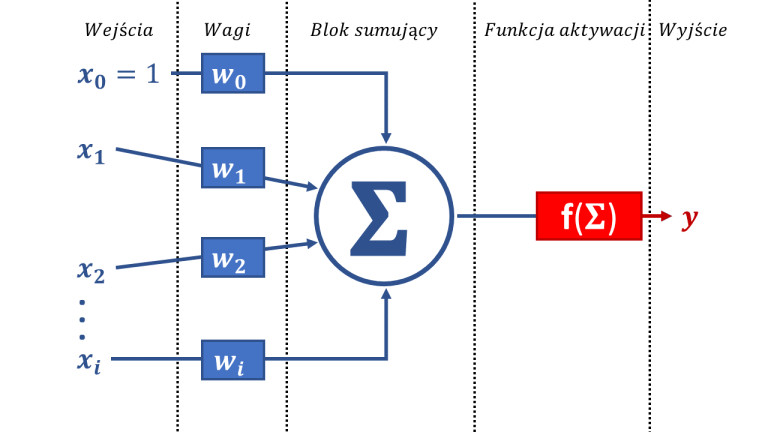
\includegraphics[width=12cm]{pages/teoria/zdjecia/sztucznyNeuron.jpg}
	\caption{Schemat pojedynczego neuronu \cite{sztucznyNeuron}}
	\label{rys:ogolnyRozwiazania}
\end{figure}


Wyjście powyższego neuronu możemy opisać wzorem:

\begin{equation}
	y = f( \sum_{i = 0}^{N}w_i x_i) = f(W^T x)
	\label{eq:rownanieNeuronu}
\end{equation}
Gdzie: $x=[1, x_1, x_2, ..., x_N]$ - to wektor sygnałów wejściowych (1 na początku wektora odpowiada
za przesunięcie), $W = [w_0, w_1, w_2, ..., w_N]$ - jest wektorem wag ($w_0$ to wartość progowa aktywacji),
$f(x)$ to wybrana funkcja aktywacji

\textbf{Najczęściej stosowane funkcje aktywacji:}

\begin{equation}
	f(x) = \frac{1}{1 + e^-x\beta} 
	\label{eq:signum}
\end{equation}

\begin{equation}
	f(x) = \frac{e^x - e^-x}{e^x + e^-x}
	\label{eq:tangensHiperboliczny}
\end{equation}

\begin{equation}
	f(x) = \begin{cases}
		1 & \text{gdy } x > 0 \\ 
		0 & \text{gdy } x < 0 
	\end{cases}
	\label{eq:skokuJednostkowego}
\end{equation}


\textbf{Wielowarstwowe sieci neuronowe}

W praktycznym zastosowaniu sieć zbudowana z jednej warstwy neuronów nie pozwoli nam na osiągnięcie satysfakcjonujących wyników.
Możemy określić dwa typy sieci pod względem liczby warstw: 
\begin{itemize}
	\item uczenie maszynowe - zazwyczaj są zbudowane z trzech warstw (ukryta-ukryta-wyjściowa), 
	\item głębokie uczenie - takie sieci posiadają dużo więcej warstw, a w skomplikowanych sieciach nawet kilkaset.
\end{itemize}

Relacje pomiędzy nimi przedstawia rysunek \ref{rys:schematAI}.
\begin{figure}[H]
	\centering
	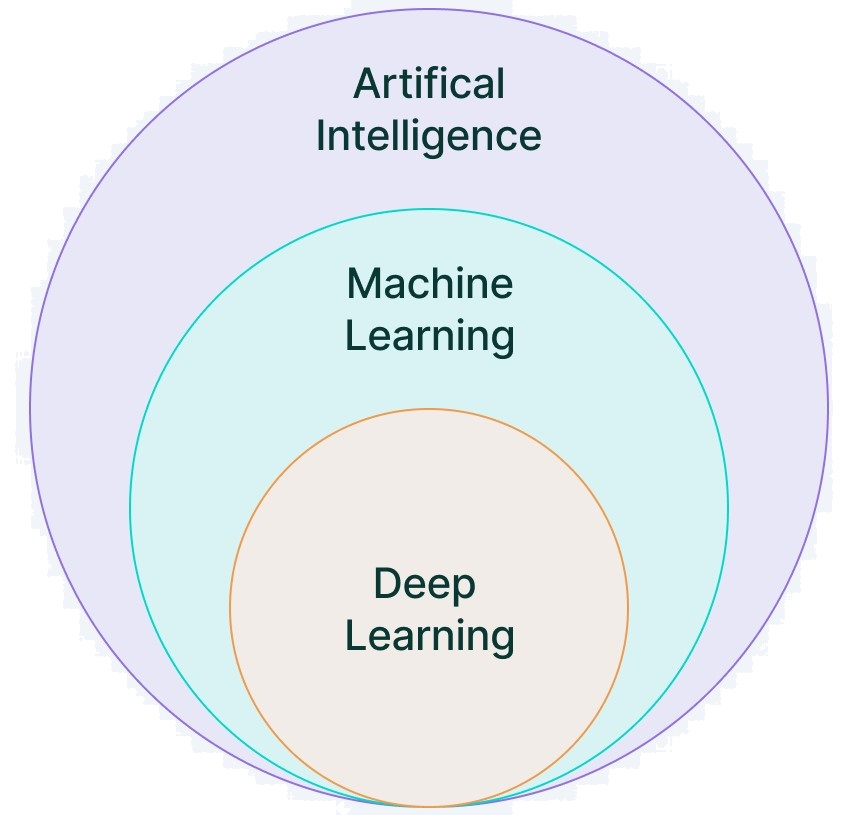
\includegraphics[width=8cm]{pages/teoria/zdjecia/schematAI.jpg}
	\caption{Relacja pomiędzy typami sieci neuronowych \cite{schematAISite}}
	\label{rys:schematAI}
\end{figure}
\subsection{Głębokie sieci neuronowe}
% klasyczne sieci neuronowe 
Ze względu na budowę głębokiej sieci neuronowej, ta bardzo dobrze radzi sobie z danymi bez struktury np. obrazy, video, dźwięk czy tekst. 
W związku z tymi cechami i wraz ze wzrostem wydajności komputerów ta jest wykorzystywana w większej ilości branż. Sieci te stosowane są 
m.in. w tłumaczeniu i analizie tekstów oraz co w tym przypadku jest ważniejsze klasyfikacji i detekcji obiektów na obrazach.

Jako że uczenie głębokich sieci neuronowych wymaga bardzo dużo czasu i wydajnych macierzy obliczeniowych powstały metody uproszczające cały ten proces. 
\subsubsection{Konwolucyjne sieci neuronowe}
Konwolucja w sieciach neuronowych bazuje na splocie i w większości przypadków oznacza nałożenie filtra na przetwarzany obraz. Operacja splotu polega na całkowaniu sygnału i wygenerowaniu wynikowego obrazu podobnego do oryginalnego.
Na podstawie tej operacji działają m.in. filtry takie jak rozmycie obrazu (filtr Gaussa) czy  algorytmy wspomagające rozpoznawanie wzorców (falki Gabora).
Operacje splotowe przyśpieszają obliczenia dzięki zmniejszeniu liczby parametrów do wyznaczenia podczas procesu uczenia. Ich dużą zaletą jest:
\begin{itemize}
	\item uwypuklenie pewnych cech obrazu co ułatwia klasyfikacje, 
	\item łączenie filtrów pozwala na wyróżnieniu wielu cech jednocześnie, 
	\item zmniejsza szum w analizowanych obrazach, 
	\item filtry "poolingowe", które redukują wymaganą ilość połączeń i neuronów co znacząco zwiększa szybkość obliczeń, 
	\item konwolucja pozwala na uniezależnienie się od pozycji wykrywanego obiektu na ekranie.
\end{itemize}
\subsubsection{Sieci rekurencyjne}

W typowej sieci neuronowej zakładamy ze wszystkie wyjścia i wejścia są niezależne od siebie co w wielu 
przypadkach jest złym założeniem (np. analiza szeregu czasowego). Sieci rekurencyjne w porównaniu do zwykłych sieci 
wyposażone są w pętle sprzężenia zwrotnego dla co najmniej jednej warstwy neuronów. Dzięki tej pętli sieć posiada 'pamięć' 
 i znacznie lepiej przewiduje wyjście dla przebiegów sekwencyjnych. Niestety przez zastosowanie sprzężenia zwrotnego, a więc zwiększenie
się liczby występowania różnych przypadków taka sieć musi być znacznie dłużej trenowana.

\subsubsection{Uczenie transferowe}

Niezależnie od stosowanego algorytmu, uczenie głębokiej sieci neuronowej jest skomplikowane i czasochłonne.
W związku z tym została opracowana metoda uczenia, polegająca na użyciu już wytrenowanych sieci i wyuczeniu
ich na nowych danych. Zaletą tego rozwiązania jest znaczne przyśpieszenie procesu uczenia, ponieważ sieć posiada już wstępnie 
ustalone wartości wag. Dodatkową zaletą przetrenowanych wag jest zmniejszenie ilości wymaganych danych do osiągnięcia zadowalających efektów. 
Zazwyczaj wytrenowane sieci są bardzo duże i posiadają miliony parametrów, nawet kilkaset kategorii i kilkadziesiąt ukrytych warstw.

\subsection{Algorytmy detekcji obiektów na zdjęciach}
W praktyce nauczenie sieci neuronowej kategoryzującej obrazy i znajdujące się na nich obiekty nie jest najtrudniejszym zadaniem stawianym 
przed takimi sieciami. Zdecydowanie większym wyzwaniem jest wskazanie dokładnej pozycji obiektu znajdującego się we wskazanym obrazie.
Szukając materiały na temat istniejących rozwiązań można natknąć się na dwa określenia: segmentacja i detekcja. 
Segmentacja polega na przydzieleniu każdego piksela obrazu do klas wyuczonych w sieci. 
Detekcja obrazu polega na znalezieniu wszystkich obiektów znanych trenowanej sieci, określeniu ich kategorii oraz wyznaczeniu 
ich pozycji.
\begin{figure}[H]
	\centering
	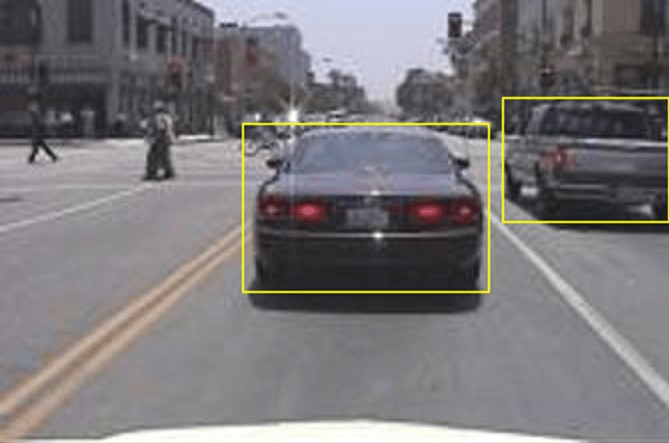
\includegraphics[width=7.5cm]{pages/teoria/zdjecia/ObjectDetectionUsingYOLOV4DeepLearningExample_01.jpg}
	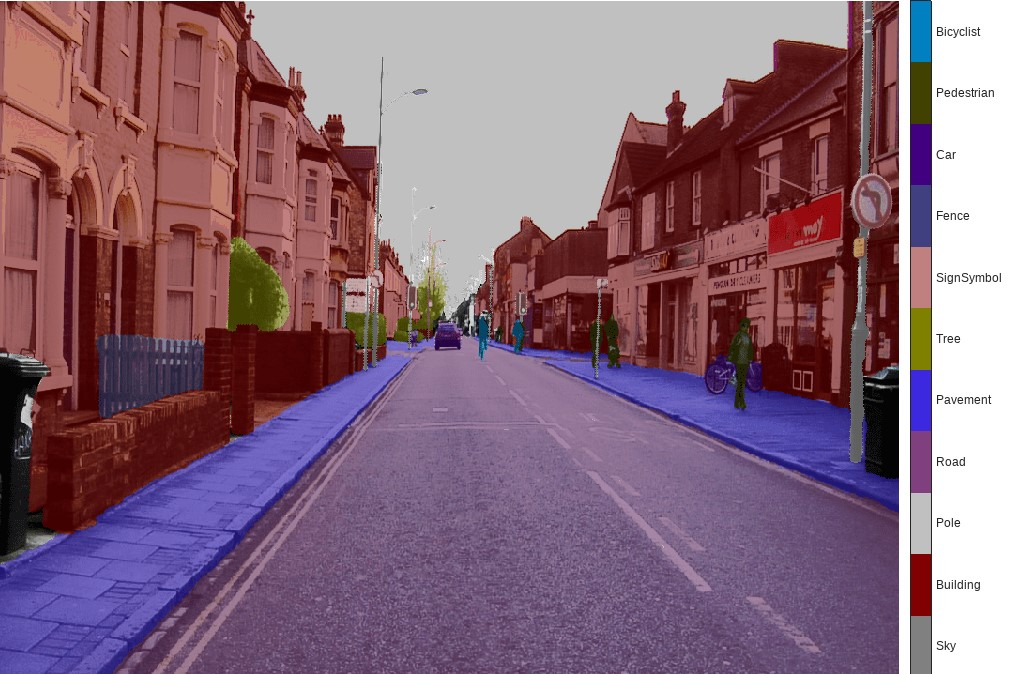
\includegraphics[width=7.5cm]{pages/teoria/zdjecia/SemanticSegmentationUsingDeepLearningExample_03.jpg}
	\caption{Pierwsze zdjęcie obrazuje detekcje obiektów, drugie to segmentacja obrazu\cite{matlabDetekcjaPrzyklad}}
	\label{rys:detekcjaVsSegemntacja}
\end{figure}

\subsubsection{Algorytmy R-CNN}
Istnieje cała rodzina algorytmów R-CNN (Regions with Convolutional Neural Network), bazujących jak sama nazwa wskazuję na splotowych sieciach neuronowych.
Rodzina ta jest grupą pierwszych algorytmów z wysokim wskaźnikiem skuteczności.

W celu rozpoznania obiektów, algorytm nakłada na oryginalny obraz 2000 regionów służących do dalszej klasyfikacji.
\begin{figure}[H]
	\centering
	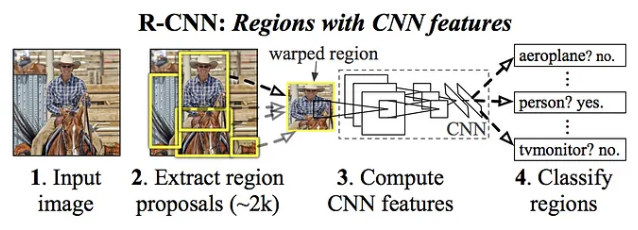
\includegraphics[width=12cm]{pages/teoria/zdjecia/strukturaSieciRCNN.png}
	\caption{Kroki działania modelu RCNN \cite{rcnnAndFRCNNTowards}}
\end{figure}
Każdy taki region trafia do sieci neuronowej zajmującej się wyodrębnieniem cech szczególnych dla danej klasy. 
Następnie wszystkie te dane trafiają do SVM (Support Vector Machine) w celu sklasyfikowania obecności obiektu w danym regionie. 
Poza klasą, sieć ta przewiduje również cztery przesunięcia, które pomagają w zwiększeniu precyzji obwiedni, szczególnie gdy obiekt znajduje się 
w kilku regionach. 

Taka sieć ma sporo wad takich jak: 
\begin{itemize}
	\item ze względu na klasyfikacje 2000 regionów na zdjęcie, uczenie trwa bardzo długo i nie może być wykonywane w czasie rzeczywistym, 
	\item bardzo długi czas przetwarzania, nawet 47s na zdjęcie, 
	\item algorytm wyszukiwania regionów jest stały i nie uczy się wraz z pozostałym algorytmem co oznacza że może też proponować złe regiony do klasyfikacji.
\end{itemize}

Kolejna wersja tego algorytmu nazwana Fast R-CNN, pozbywa się generowania za każdym razem 2000 regionów, które potem były przetwarzane. 
W tej wersji wykorzystano kolejną sieć neuronową do generowania splotowej mapy obiektów. 
Dalej na podstawie tej mapy identyfikowane są proponowane regiony, które są skalowane do jednego, stałego rozmiaru i klasyfikowane przez kolejną sieć neuronową.
Dzięki temu algorytm nie przetwarza za każdym razem 2000 regionów a operacja splotu wykonywana jest tylko raz. 

\begin{figure}[H]
	\centering
	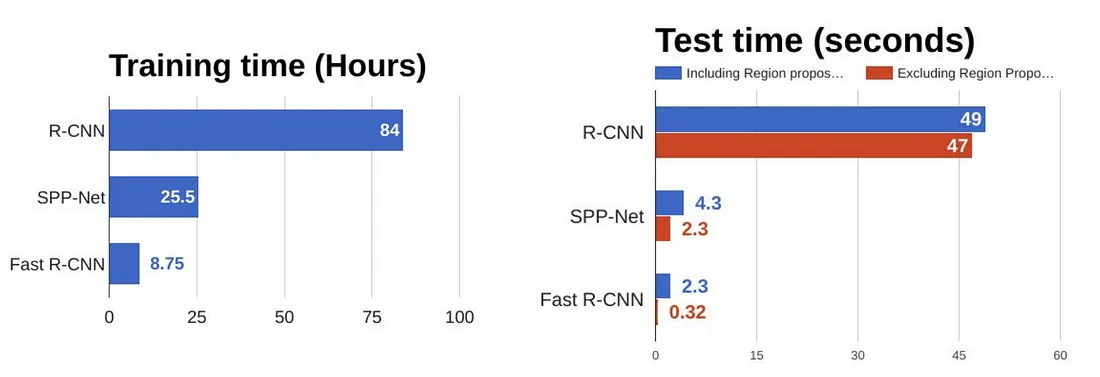
\includegraphics[width=15cm]{pages/teoria/zdjecia/RCNNvsFRCNNPorownanie.png}
	\caption{Porównanie wydajności rodziny algorytmów R-CNN \cite{rcnnAndFRCNNTowards}}
	\label{rys:porownanieRCNN}
\end{figure}
Rysunek \ref{rys:porownanieRCNN} przedstawia porównanie wydajności w kolejnych wersjach modeli do detekcji obiektów. 
Widoczna jest duża różnica w czasie przetwarzania obrazu pomiędzy pierwszą i kolejnymi dwoma wersjami algorytmów.

\subsubsection{Szybka detekcja przy pomocy YOLO}

Algorytm YOLO (You only look once) w przeciwieństwie do pozostałych algorytmów może działać w czasie rzeczywistym.
Wszystkie tradycyjne metody detekcji obiektów cały proces dzielą na kilka odrębnych faz, a YOLO wykonuje analizę i predykcje obiektów jednocześnie.
Działanie algorytmu można rozpisać w kilku krokach: 
\begin{itemize}
	\item  wejściowy obraz dzielony jest na siatkę komórek o rozmiarze SxS, 
	każda taka komórka odpowiedzialna jest za przewidywanie obiektów znajdujących się w jej obszarze,
	\item dalej dla każdej wygenerowanej ramki wykonywana jest predykcja,
	poprzez wyznaczenie B obiektów i współrzędnych prostokąta otaczającego obiekt. 
	Wektor wyjściowy ma rozmiar B*5 wartości, ponieważ cztery pola zarezerwowane są dla rozmiaru i pozycji prostokąta, a 
	piąte, logiczne oznacza czy w danej komórce znajduje się obiekt,
	\item po przewidzeniu ramek dla wszystkich komórek, przy pomocy techniki NMS (Non-maximum suppression) lokalizowane i usuwane 
	są duplikaty tych samych obiektów,
	\item ostatecznie na podstawie poprzednich kroków generowane są wyniki w postaci otaczających dany obiekt ramek, wykrytych etykiet i ich prawdopodobieństwa.
\end{itemize}

Dzięki takiemu podejściu wykrywanie obiektów przy pomocy YOLO jest dużo szybsze, a równocześnie równie skuteczne w porównaniu do tradycyjnych metod.

\begin{figure}[H]
	\centering
	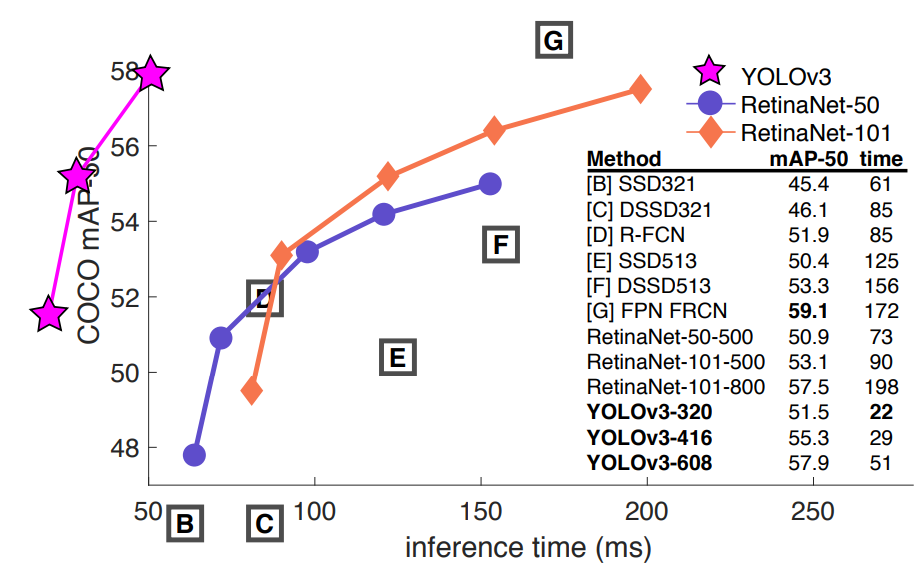
\includegraphics[width=14cm]{pages/teoria/zdjecia/wykresDzialaniaYOLO.png}
	\caption{Zdjęcie porównujące szybkość i skuteczność różnych algorytmów detekcji obiektów. \cite{yoloV3ArtAutora}}
	\label{rys:porownanieAutora}
\end{figure}

Na rysunku \ref{rys:porownanieAutora} widać, że algorytm YOLO w wersji trzeciej jest zdecydowanie szybszy od pozostałych prezentowanych przykładów równocześnie zachowując podobną skuteczność wykrywania.
Dla przykładu algorytm R-FCN przetwarza jeden obraz w czasie około 85ms ze skutecznością 51,9mAP, a najgorszy przypadek dla algorytmu YOLO potrzebuje już tylko 55ms i osiąga skuteczność 57,9mAP.
Na podstawie przedstawionego przykładu możemy zauważyć, że omawiany algorytm jest zdecydowanie lepszy w rozwiązaniach mających pracować w czasie rzeczywistym.

Parametr mAP (mean Average Precision) jest miarą używaną do porównywania różnych modeli detekcji obiektów na obrazie. Wskaźnik ten wyznaczony jest dla wszystkich klas danych obiektów co oznacza, 
że uwzględnia ogólną wydajność modelu, a nie skuteczność tylko jednej kategorii. Im wyższa wartość tym lepsza wydajność detekcji.